\documentclass[notitlepage, 12pt]{report}
\usepackage[utf8]{inputenc}
\usepackage[T1]{fontenc} % makes the angle brackets display properly
\usepackage[margin=1in]{geometry}
\usepackage{graphicx}
\usepackage{enumitem}
\usepackage{helvet}
\usepackage{wrapfig}
\usepackage{float}
\usepackage{tabularx}
\usepackage[export]{adjustbox}
\usepackage{fontspec}
\usepackage{xcolor}
\usepackage{titling} % https://tex.stackexchange.com/questions/591/removing-vertical-space-inside-maketitle/593
\renewcommand{\familydefault}{\sfdefault}

\graphicspath{{images/}}

\title{Criterion C: Development}
\definecolor{msblue}{HTML}{5AB5D8}
\makeatletter

\begin{document}
% Title
\centerline{\textcolor{msblue}{
		\fontspec{Cambria}\textbf{\fontsize{13}{13}\@title}
	}}
\bigskip

My timeblocker program is written using a client-server architecture. The client is a website frontend written using HTML, CSS, and TypeScript (a statically-typed superset of JavaScript). The server is a Node.js backend with a PostgreSQL database.

\section*{Frontend}
The frontend is a single-page application built with Vue, a JavaScript framework for building user interfaces. The files for the frontend are all contained within the `frontend/` folder.

\section*{Significant files/folders:}
\begin{tabularx}{\textwidth}{
		@{}
		p{0.3\linewidth}
		X
	}
	% https://tex.stackexchange.com/a/57709
	\centerline{\adjustbox{valign=t}{
			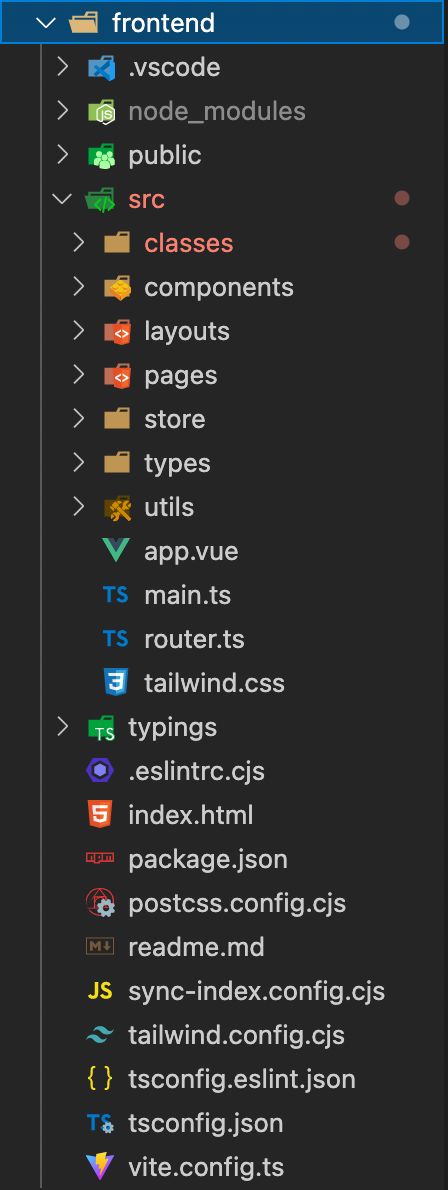
\includegraphics[width=0.3\textwidth]{frontend-files.png}
		}}
	 &
	\begin{itemize}[label={}, leftmargin=5pt]
		\item \textbf{public:} Assets that are hosted on the website as-is (e.g. the favicon).
		\item \textbf{src/:} The main website source code.
		      \begin{itemize}[label={}]
			      \item \textbf{classes/:} Frontend’s OOP classes.
			      \item \textbf{components/:} Vue components.
			      \item \textbf{layouts/:} UI templates reused across multiple pages.
			      \item \textbf{pages/:} Website pages.
			      \item \textbf{store/:} Global data store.
			      \item \textbf{types/:} TypeScript types.
			      \item \textbf{utils/:} Various utility functions.
			      \item \textbf{app.vue:} Main Vue component.
			      \item \textbf{main.ts:} Entrypoint for website scripts.
			      \item \textbf{router.ts:} Website routing configuration.
			      \item \textbf{tailwind.css:} Loads TailwindCSS styles.
		      \end{itemize}
		\item \textbf{index.html:} Website entrypoint.
		\item \textbf{Configuration files (*.cjs, *.json, vite.config.ts):} Configuration files for various frontend development tools.
	\end{itemize}
\end{tabularx}
\section*{Development}
To develop my program, I used various build tools from the JavaScript ecosystem.
For the frontend, I used Vite, a build tool that uses Hot Module Reload to update the site without needing to refresh the page and thus resetting the page state.
When building the site for production, Vite uses Rollup to bundle all the website assets which is what is served to the client when they visit the public website hosted on GitHub pages.

\section*{User Interface}
\begin{tabularx}{\textwidth}{
		@{}
		p{0.3\linewidth}
		X
	}
	\centerline{\adjustbox{valign=t}{
			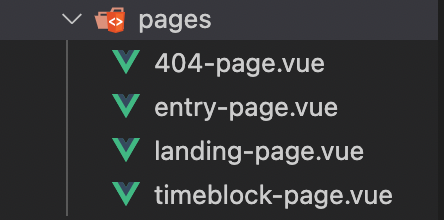
\includegraphics[width=1\linewidth]{frontend-pages-folder.png}
		}}
	 &
	The code responsible for the user interface is stored under the src/pages folder.
	The .vue file extension indicates Vue Single-File Components, or SFCs for short.
	These files contain all the necessary HTML, CSS, and JavaScript to render a component part of a dynamic user interface.
\end{tabularx}

\vspace{10pt}

% https://tex.stackexchange.com/questions/205086/do-not-indent-a-tabular
\noindent\begin{tabularx}{\textwidth}{
		@{}
		X
		p{0.6\linewidth}
		@{}
	}
	In each Vue SFC, there are three root tags: the <script> tag, the <template> tag, and the <style> tag. The <script> tag contains the JavaScript that is executed when the component is initialized for the first time. The <template> tag contains the HTML that defines the structure of the component, and the <style> tag contains the CSS that is used to style the component.
	 &
	\centerline{\adjustbox{valign=t}{
			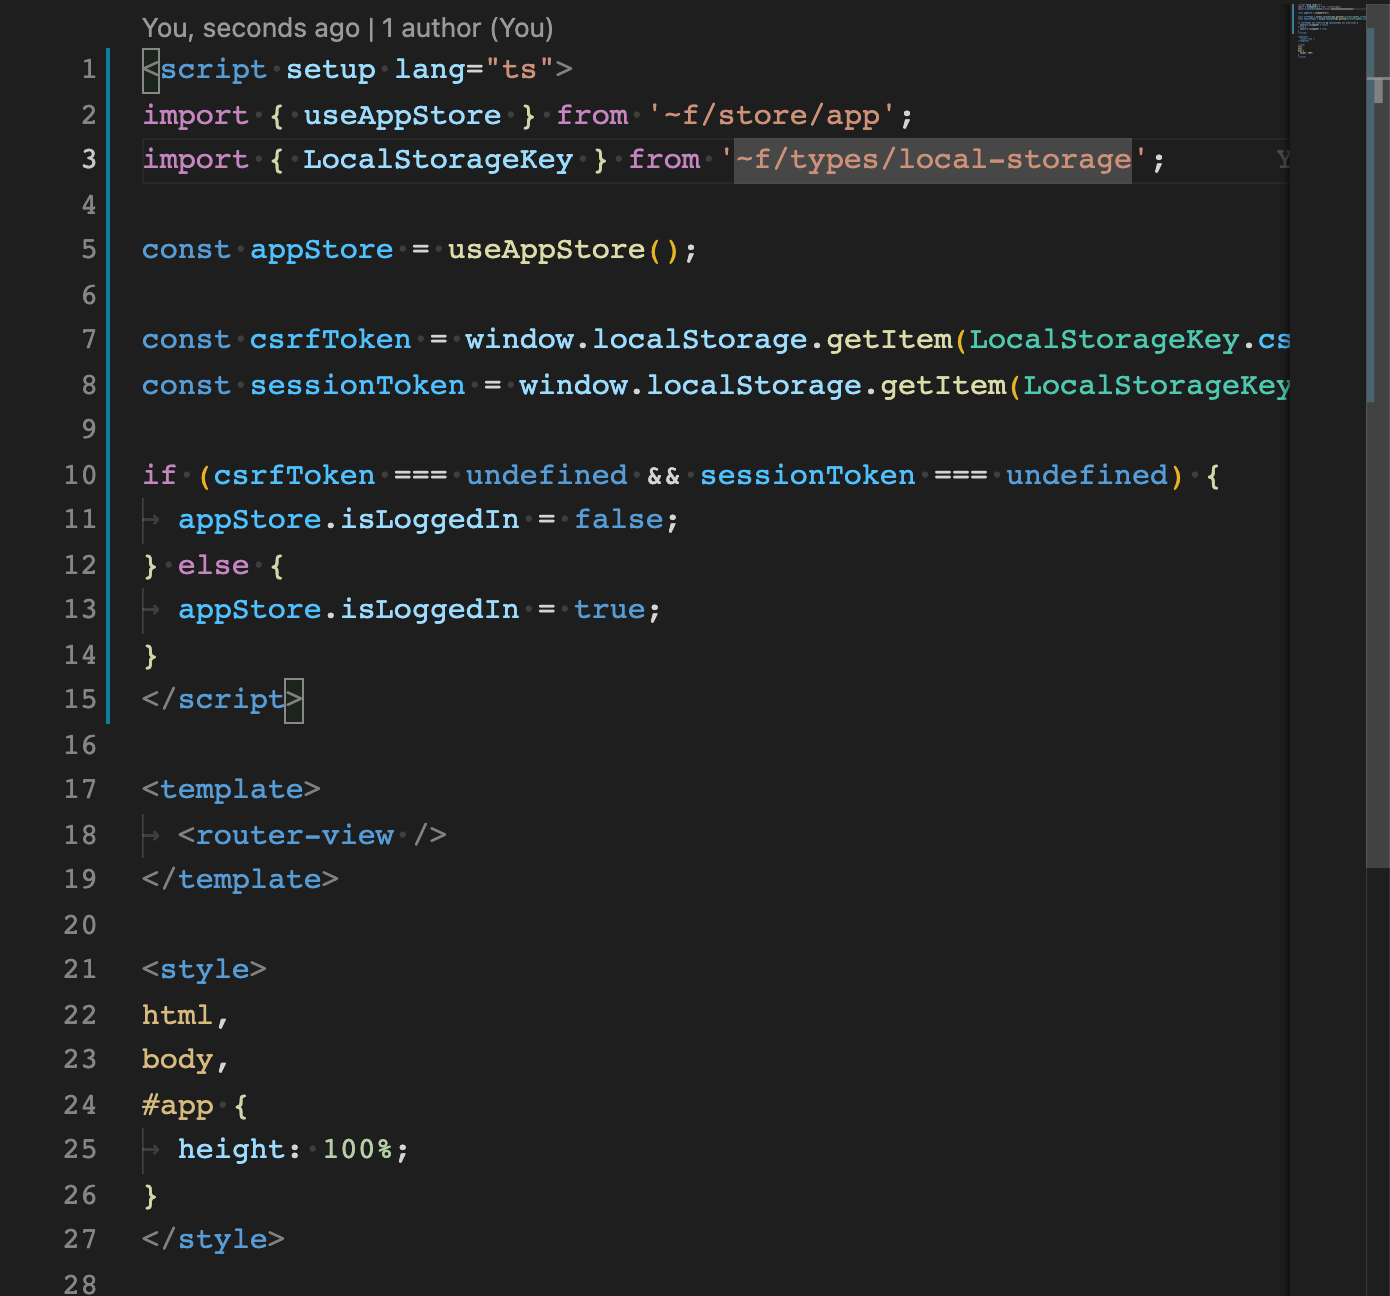
\includegraphics[width=0.6\textwidth]{frontend-vue-sfc.png}
		}}
\end{tabularx}

Most of the SFCs don’t contain a <style> tag because the CSS styles are primarily contained within the HTML through TailwindCSS’s utility classes. TailwindCSS is a CSS framework that provides flexible utility classes for making it easier to style HTML. In addition, I used a Tailwind library known as daisyUI that provides out-of-the-box styled components for common HTML components.

\section*{Landing Page}
The landing page is the page that users are brought to when they first visit the website. It contains a hero banner with a call to action. On the top right, if the user is logged in, there will be an “Open Timeblock” button that directs them to their timeblock, and if they aren’t logged in, there will be a “Sign up” and “Login” button that allow them to sign up for log into an account.

\section*{Entry Page}

\section*{Registration}
The user must create an account to use the program. They need to enter their email and password, and a confirmation email will be sent to confirm they entered their email correctly (which is crucial for emails like password reset requests). In addition, the registration page comes with a captcha to prevent attackers from spamming unwanted registration requests.

\section*{Authentication}
Once a user registers or logs in, the server sends the client an httpOnly cookie containing a session token and a CSRF token to prevent Cross-Site Request Forgery attacks. The httpOnly cookie prevents JavaScript from accessing the cookie, minimizing the damage of Cross-Site Scripting attacks.

\section*{Timeblock Page}
The timeblock page consists of two main views: the “Task Dock” and the “Timeblock Calendar.”

The task dock contains all the user’s tasks, and the user has the option to add and delete tasks. The user can add a task by pressing on the “Add Task” button. The calendar contains all the “task blocks,” which represent chunks of time dedicated to a user’s task. The user can toggle the task dock on and off by pressing the menu in the top left. To create a new task block, the user can drag one of their existing tasks onto the calendar. Then, a new task block will appear on the calendar that the user can resize or drag to a different time slot.

On the right side of the timeblock calendar, there is a plus icon that allows the user to add a new timeblock column. Timeblock columns are used for creating multiple versions of a timeblock, as it’s common for users to experience interruptions in their day and need to recreate their timeblock.

\section*{Backend}
The backend uses tRPC, a TypeScript library for defining type-safe server routes, and Fastify, a low overhead web framework for Node.js. Significant files/folders include:

\noindent\begin{tabularx}{\textwidth}{
		@{}
		p{0.3\linewidth}
		X
	}
	\adjustbox{valign=t}{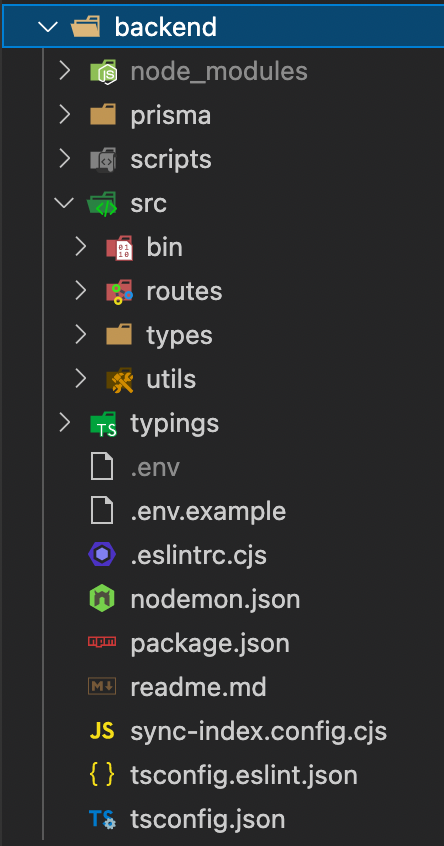
\includegraphics[width=0.3\textwidth]{backend-files.png}}
	 &
	\begin{itemize}[label={}, leftmargin=5pt]
		\item	\textbf{prisma/:} Database models and configuration files for the Prisma ORM.
		\item	\textbf{src/:} Main backend source code.
		\item	\textbf{bin/:} Scripts that should be executed to start the server.
		\item	\textbf{routes/:} tRPC route definitions.
		\item	\textbf{types/:} TypeScript types.
		\item	\textbf{utils/:} Various utility functions.
		\item	\textbf{.env:} Environment secrets (should not be public!)
		\item	\textbf{Configuration files (*.cjs, *.json):} Configuration files for various backend development tools.
	\end{itemize}
\end{tabularx}

\section*{Database Models}
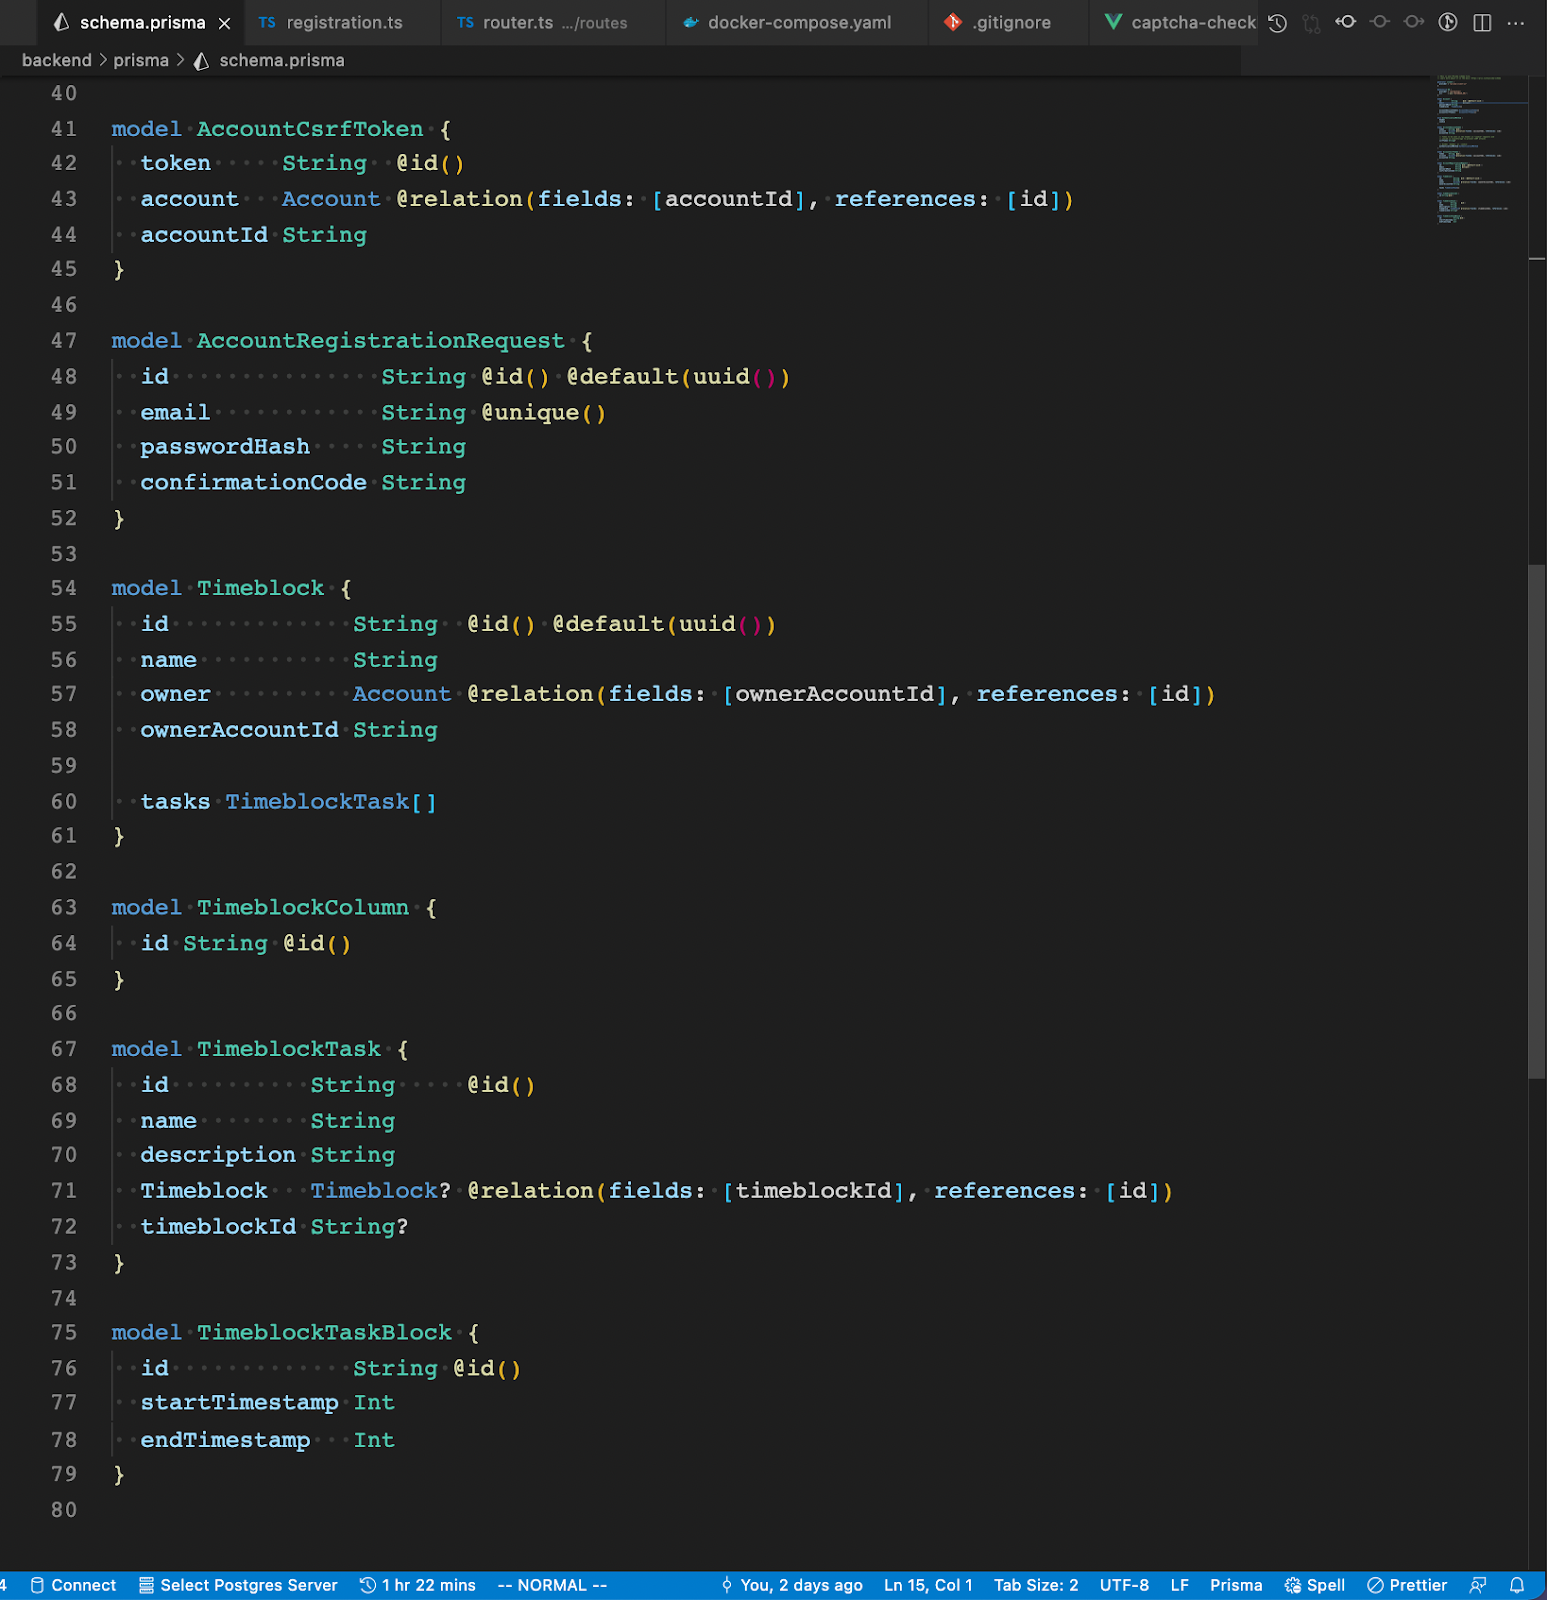
\includegraphics[width=1\textwidth]{backend-database-models.png}

\section*{tRPC Routes}
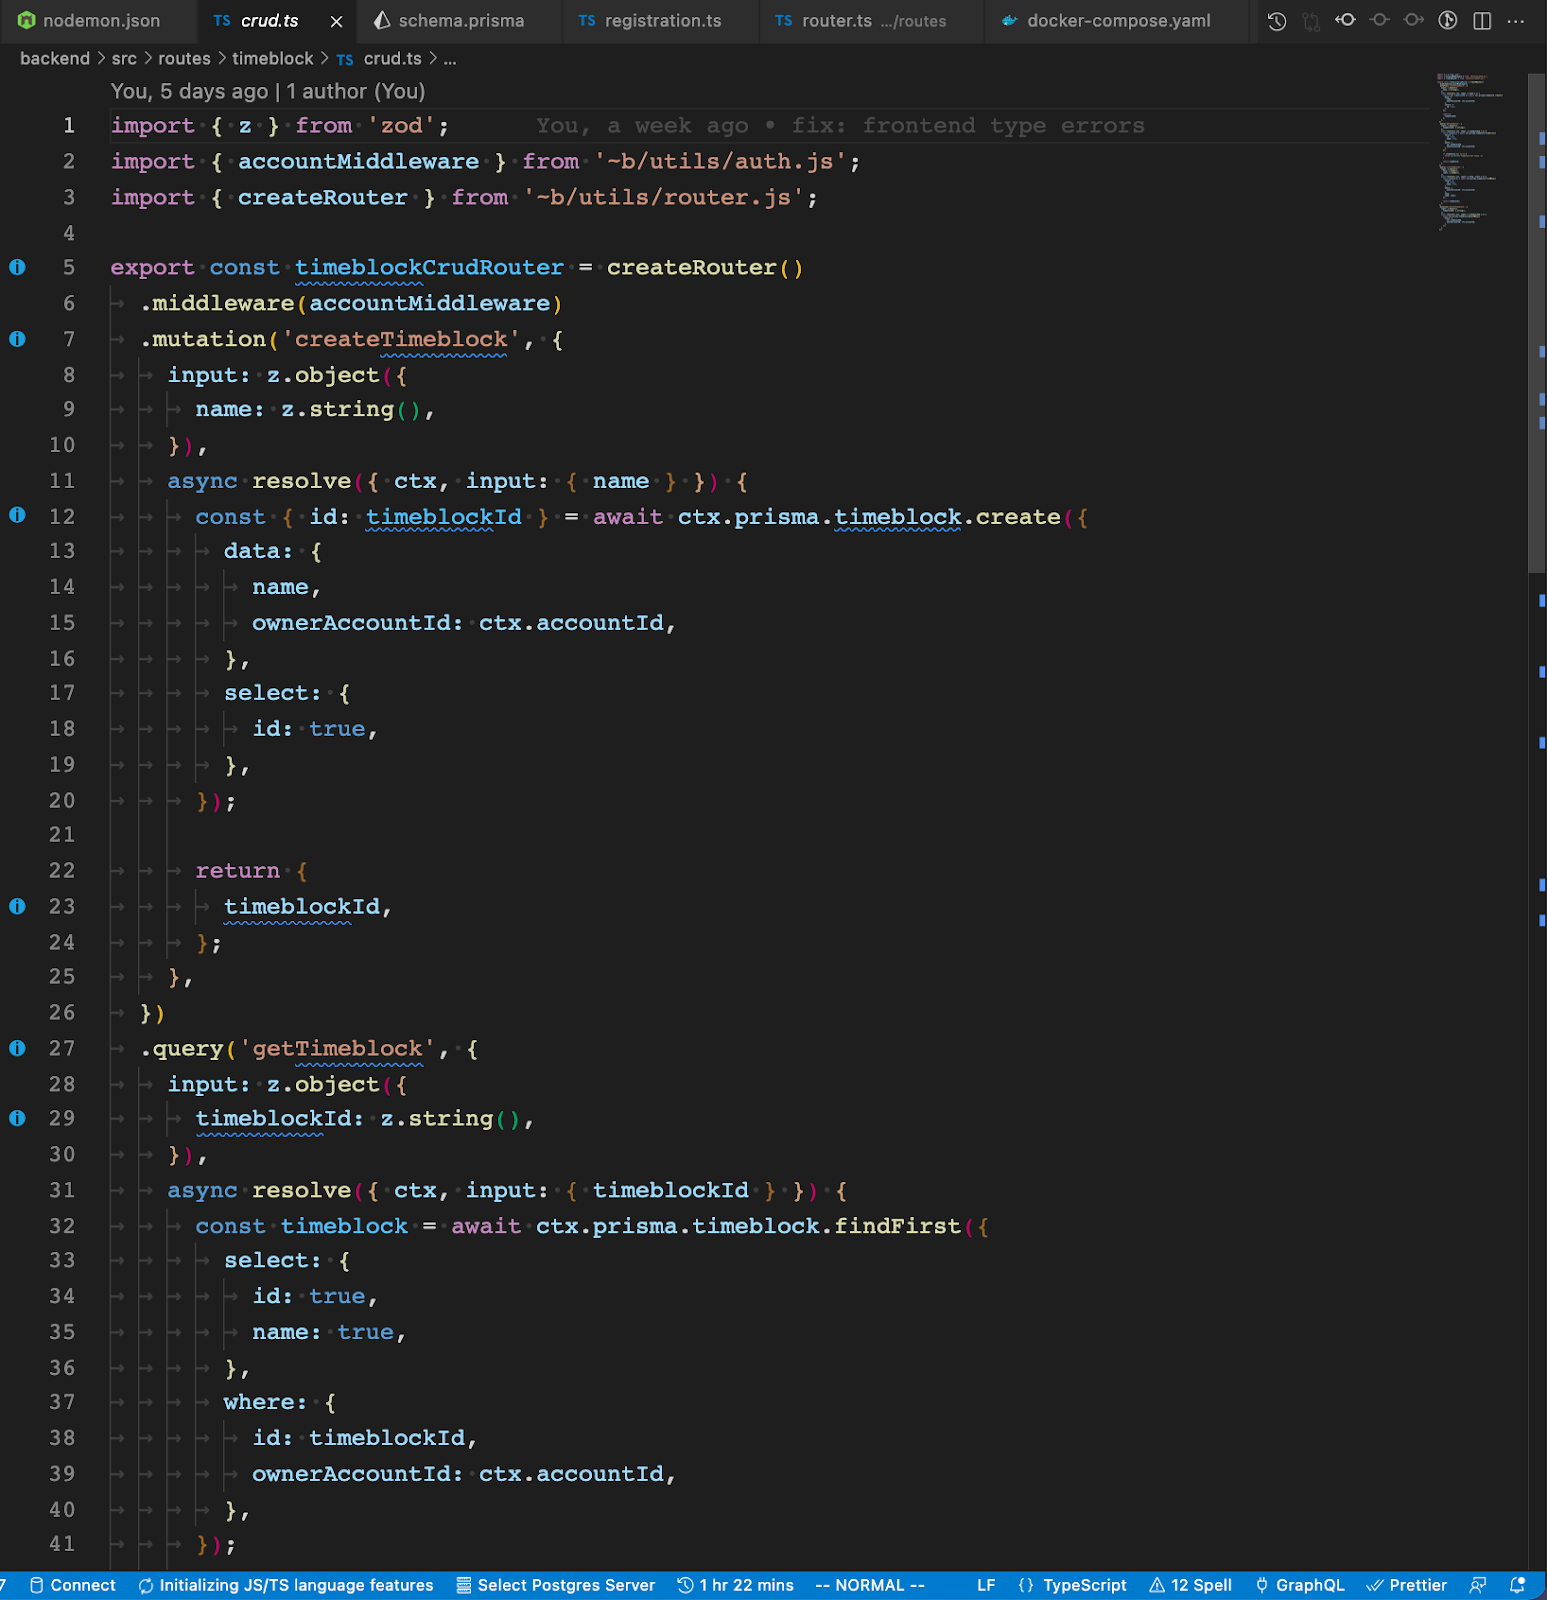
\includegraphics[width=1\textwidth]{backend-trpc-routes.png}

\end{document}
